\subsection{Revisions and Commits}
\label{section_revisions_and_commits}
\renewcommand{\figurename}{Diagram}
Every Subversion revision and every Git commit consists of:
\begin{itemize}
\item Metadata, which includes author, message, date and reference to the previous revision or to the parent commits. While
concepts of the parent commit and that of previous revisions have different semantic in their details, both represents history line, 
i.e. previous states of repository preceding this commit.
\item Contents, which might be described explicitly or as a set of modifications applied to the previous contents state.
\end{itemize}
Following sections outlines general translation rules used to translate Subversion revision to Git commits and Git commit
to Subversion revision. This chapter describes general translation rules for revisions and commits, while further chapters provides all the 
necessary details for processing of the special cases.
\subsubsection{Translating Subversion Revision to Git Commits}
Every Subversion revision is translated to one or more Git commits and,
when required by the translation rules, to the creation or deletion of Git reference objects (Git branches and tags).
\\\\
Subversion revision translation is performed in multiple stages.
First, paths affected by Subversion revision are grouped by the branch or tag these paths belong to. The
reason for this grouping is that with Subversion, a user can made modifications on serveral branches or tags 
in the same revision. This is not possible with Git. Hence, the translation may require more than one commit in the Git repository, 
each commit modifing single branch.
\\\\
Consider the following modifications made in a single Subversion revision:
\\\\
M \textbf{/trunk}/file.txt\\
M \textbf{/branches/branch1}/file2.txt\\
D \textbf{/branches/branch1}/file3.txt\\
A \textbf{/tags/tag1} copied from \textbf{/trunk} at r3\\

Affected paths will be grouped by affected branches into these three groups:
\begin{enumerate}
\item \textbf{/trunk}:\\
M file.txt
\item \textbf{/branhces/branch1}:\\
M file2.txt\\
D file3.txt
\item \textbf{/tags/tag1}:\\
  copied from \textbf{/trunk} at r3
\end{enumerate}
Then, each group of modifications is translated either to the Git commit or to
the Git branch or tag deletion or creation. 
\begin{center}
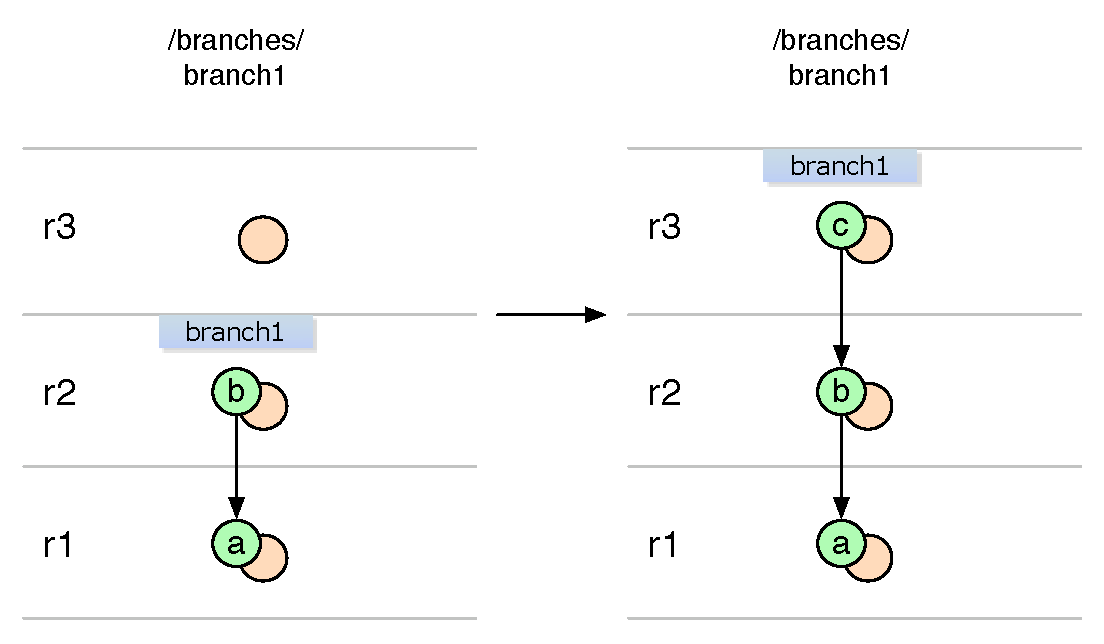
\includegraphics[width=\textwidth]{img/diagrams/single_change_svn_to_git.pdf}%
\captionof{figure}{Subversion revision being translated to Git commit.}
\label{single_change_svn_to_git}%
\end{center}
To translate regular modification of multiple paths within specific branch (/branches/branch1) at certain revision (r3), 
Translator goes through the following steps: 
\begin{enumerate}
	\compactlist
	\item Creates commit \emph{c} with tree object corresponding to /branches/branch1@r3 subdirectory content.
	\item Commit \emph{c} has author ident and committer ident set to the author of the revision r3.
	\item Commit \emph{c} has the date set to that of the revision r3.
	\item Commit \emph{c} has the message set to that of the revision r3.
	\item Commit \emph{c} has parent commit set to commit \emph{b} which corresponds to revision r2, i.e. previous modification of branch1.
	\item And finally Translator updates reference /refs/heads/branch2 to the created commit \emph{c}.
\end{enumerate}

Some modifications, in particular those affecting branches and tags directories in Subversion repository, may
result in the Git branches or tags being created, deleted or modified in Git repository. Refer to the section \ref{section_branches_and_tags} for the corresponding translation rules. 

\subsubsection{Translating Git Commit to Subversion Revision}
Every Git commit is translated to a single Subversion revision. Subversion revision might also be an outcome of 
the Git reference objects (branches and tags) translation. There is always a Subversion revision
which corresponds to the Git commit, but not every Subversion revision created by the Translator has 
corresponding Git commit.
\begin{center}
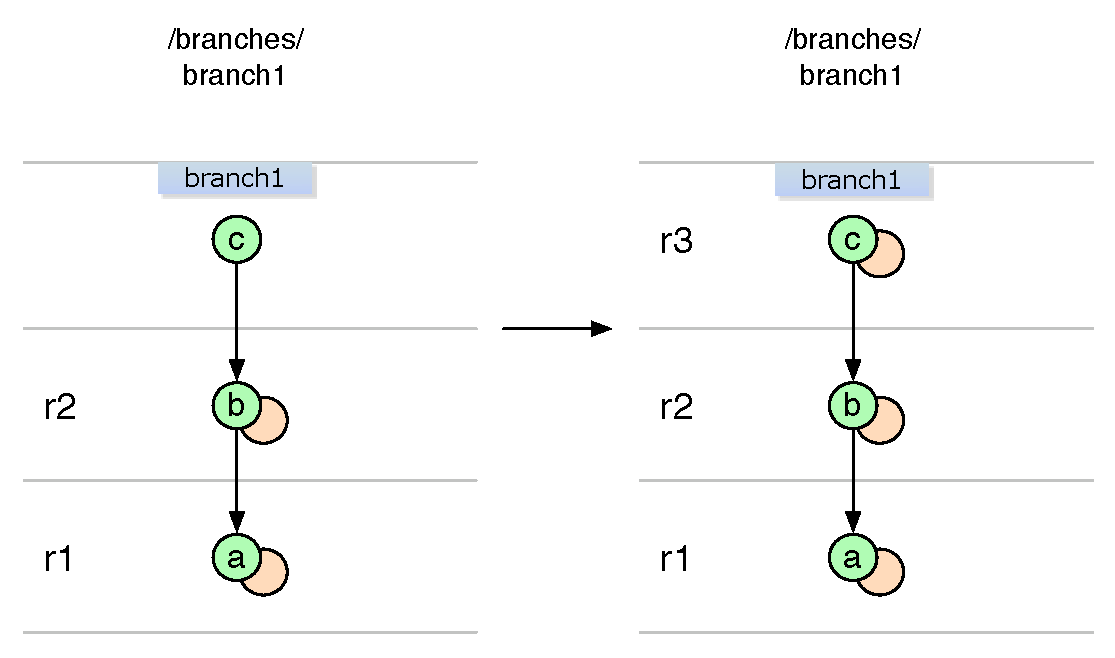
\includegraphics[width=\textwidth]{img/diagrams/single_change_git_to_svn.pdf}%
\captionof{figure}{Git commit being translated to Subversion revision.}
\label{single_change_git_to_svn}%
\end{center}

To translate regular Git commit (\emph{c}) on a particular branch (\emph{branch1}), Translator does 
the following:
\begin{enumerate}
	\compactlist
	\item Creates \emph{revision r3} in which /branches/branch1 directory content corresponds to the tree object of the Git \emph{c} commit. 
	\item Revision r3 has the author set to the author ident of the Git commit \emph{c}.
	\item If the latest revision of Subversion repository before translation had date before Git commit \emph{c} creation date, this creation date is used for revision r3, otherwise the date of committing revision r3 is used.
	\item Revision r3 has commit message set to the message of the Git commit \emph{c}.
\end{enumerate}

Some of the translation scenarios includes setting of additional properties on files and directories 
in Subversion repository, depending on the specific changes in the original Git commit contents and 
on the particular ancestors set of the original Git commit. These aspects of contents translation are considered in the further chapters of
this specification. Metadata translation rules are common for all translation scenarios.